\section{Pianificazione}
La pianificazione di progetto viene suddivisa nelle seguenti fasi:
\begin{enumerate}

	\item \textbf{Analisi};
	\item \textbf{Progettazione della technology baseline};
	\item \textbf{Codifica del Proof of Concept};
	\item \textbf{Progettazione di dettaglio e codifica};
	\item \textbf{Completamento e raffinamento delle funzionalità};
	\item \textbf{Validazione e collaudo}.
\end{enumerate}

Le fasi \textit{(3), (4)} e \textit{(5)} sono di supporto al gruppo in modo da rispettare le scadenze per lo sviluppo del progetto (riportate a \S 1.4.3). La presenza di tali fasi ha lo scopo di aumentare la comprensione del documento e non deve essere considerata per la scansione degli incrementi, in modo da non collidere con la natura del modello di sviluppo scelto. Per questo motivo non sono citate in \S 5 e \S 6.
\subsection{Analisi}
Questa fase comincia con la presentazione dei capitolati d'appalto e termina con la data di consegna per la \textit{Revisione dei Requisiti}, ovvero dal 05-11-2020 al 11-01-2021.
In questo periodo verranno redatti tutti i documenti necessari e verrà fatta un'analisi approfondita del capitolato scelto dal gruppo \Gruppo{}.

\subsubsection{Obiettivi}
Organizzazione interna del team e stesura di tutti i documenti.

\subsubsection{Periodi e attività}
La pianificazione di questa fase è stata organizzata nei seguenti periodi:
\begin{itemize}
\item \textit{Dal 05-11-2020 al 04-12-2020}: individuazione degli strumenti per la comunicazione interna e discussione dei capitolati proposti. Inizio della stesura dello \SdF{} con \glo{milestone} il 10-12-2020;

\item \textit{Dal 05-12-2020 al 22-12-2020}: stesura delle \NdP{} e del \PdP{} e iniziata inoltre la stesura dell'\AdR{}. Il 22-12-2020 il gruppo ha fissato una milestone\glo{} per la verifica dei prodotti;

\item \textit{Dal 23-12-2020 al 05-01-2021}: il gruppo si dedica all'\AdR{} e al contempo inizia la stesura del \PdQ{}. Il 05-01-2020 il gruppo fissa un'ulteriore milestone\glo{} per verificare che tutti i documenti siano stati completati correttamente;

\item \textit{Dal 06-01-2021 al 11-01-2021}: si svolge attività di verifica su tutti i documenti, si completano eventualmente documenti in ritardo. Si uniformano tutti i documenti stando alle regole stabilite nelle \NdP{}.
\end{itemize}

\begin{landscape}

\begin{figure}[h]
	\centering
	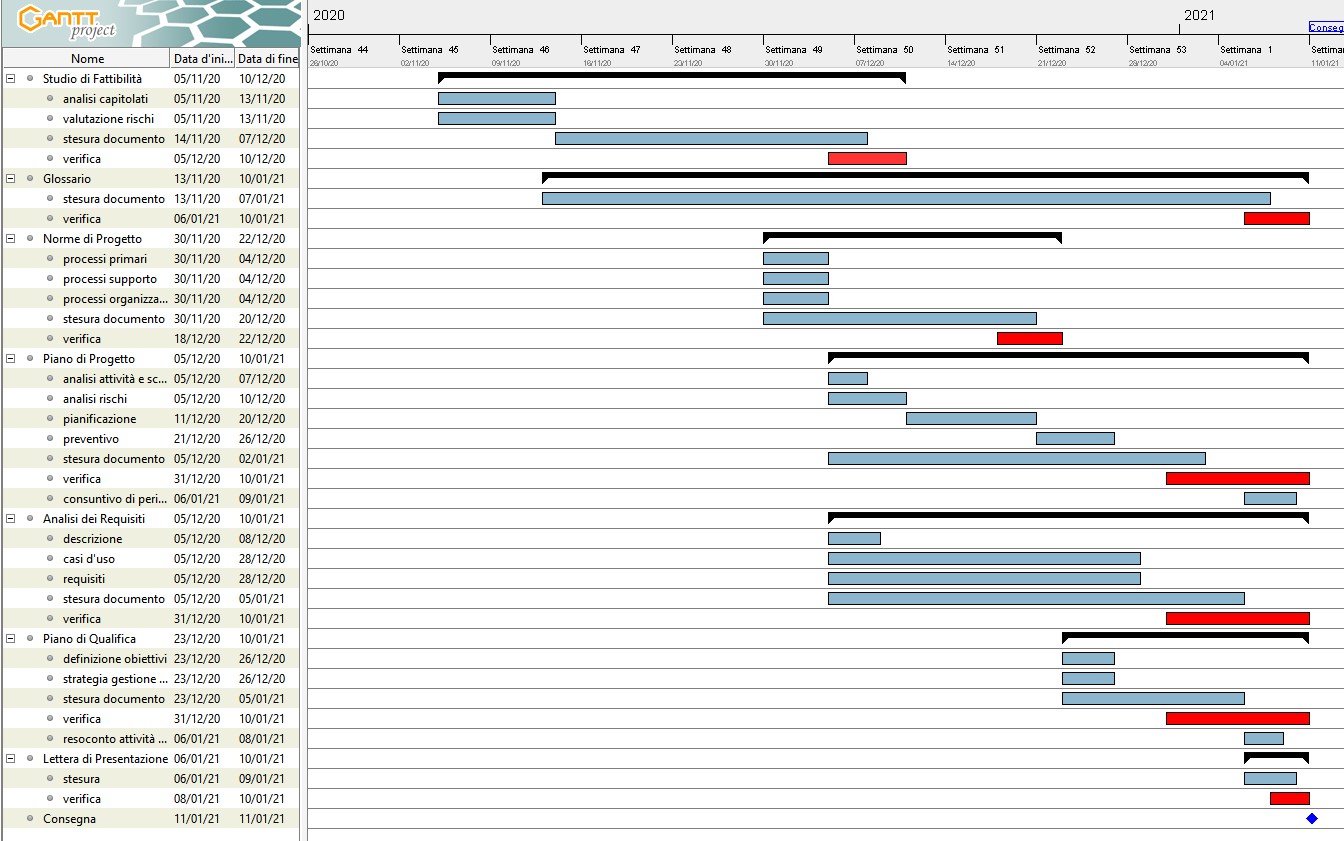
\includegraphics[width=\linewidth]{Images/GanttPianificazioneAnalisi.PNG}
	\caption{Diagramma di Gantt dell'attività di analisi}
\end{figure}

\end{landscape}




\newpage
\subsection{Progettazione della Technology Baseline}
A causa della concomitanza con la sessione accademica, il team ha fissato la prima \glo{milestone} al termine di questo periodo. 
\subsubsection{Obiettivi}
Il gruppo dovrà aver iniziato lo studio delle tecnologie per la \textit{Technology Baseline}, oltre ad aver controllato buona parte della documentazione.
\subsubsection{Periodi e attività}
Questo periodo è unico e ha inizio il giorno 18-01-2021, successivamente alla revisione dei requisiti, con termine fissato per il giorno 07-02-2021. Comprende attività di: 
\begin{itemize}
\item \textbf{Incremento e verifica dei documenti}: se fosse necessario, i documenti prodotti dal team verranno integrati;
\item \glo{\textbf{Technology Baseline}}: viene fatta un'analisi ad alto livello per comprendere le tecnologie coinvolte.
\end{itemize}

\begin{figure}[h]
	\centering	
	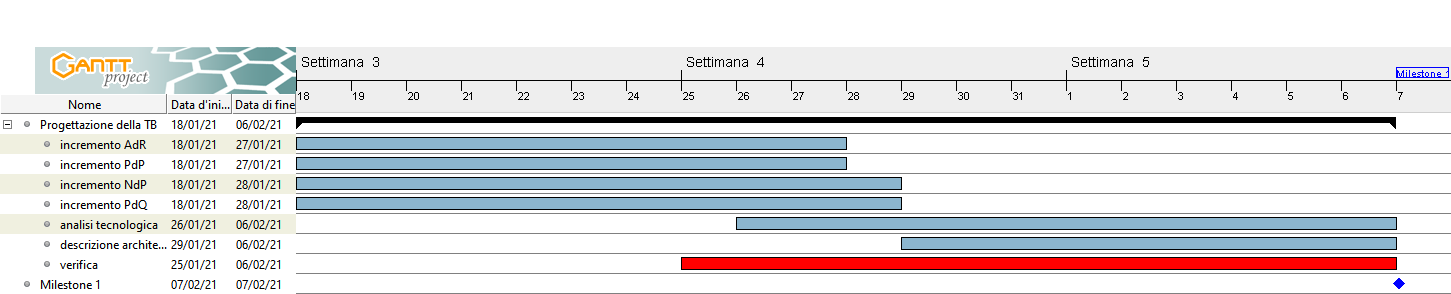
\includegraphics[width=\linewidth]{Images/GanttPianificazioneProgettazioneTB.PNG}
	\caption{Diagramma di Gantt dell'attività di progettazione della Technology Baseline}
\end{figure}
\newpage
\subsection{Codifica del Proof of Concept}
Questa fase comincia subito dopo il termine della precedente e finisce con la data di consegna per la \textit{Revisione di Progettazione}, ovvero dal 08-02-2021 al 01-03-2021. Lo scopo di questa fase è quello di consolidare la progettazione della Techonology Baseline attraverso l'implementazione di un Proof Of Concept.
\subsubsection{Incremento I}
\paragraph{Obiettivi}
\begin{itemize}
\item Sviluppo di una prima bozza dell'\glo{UI} ;
\item Implementazione di un componente per il caricamento dei dati nel sistema attraverso un file in formato \glo{CSV} \textbf{[UC1.1.1]};
\item Implementazione di una sezione per la selezione delle dimensioni da utilizzare \textbf{[UC2]}.
\end{itemize}
		
\paragraph{Periodi e attività} \mbox{}\\\mbox{}\\
Questo incremento si compone di un unico periodo, dal 08-02-2021 al 18-02-2021, con milestone fissata per l'ultimo giorno. Comprende attività di:
\begin{itemize}
\item \textbf{Verifica dei documenti};
\item \textbf{Studio delle tecnologie:} studio della documentazione delle librerie \glo{D3.js} e \glo{React};
\item \textbf{Progettazione:} progettazione di un componente per il caricamento dei dati e uno per la selezione delle dimensioni;
\item \textbf{Codifica:} codifica dei componenti progettati;
\item \textbf{Verifica software:} verifica sulle funzionalità software aggiunte.
\end{itemize}

\subsubsection{Incremento II}  
\paragraph{Obiettivi}
\begin{itemize}
\item Implementazione della visualizzazione \glo{Scatter Plot Matrix} \textbf{[UC5.1]};
\item Aggiunta di alcuni controlli per la configurazione dei parametri relativi alla visualizzazione precedentemente implementata  \textbf{[UC6.1]}. 
\end{itemize}			
	
\paragraph{Periodi e attività} \mbox{}\\\mbox{}\\
Questo incremento si compone di un unico periodo, dal 18-02-2021 al 01-03-2021, con milestone fissata per l'ultimo giorno. Comprende attività di:
\begin{itemize}
\item \textbf{Studio delle tecnologie:} studio più approfondito della documentazione delle tecnologie interessate;
\item \textbf{Progettazione:} progettazione di un componente per la visualizzazione \glo{Scatter Plot Matrix} e del collegamento tra server, \glo{database} e \glo{web app};
\item \textbf{Codifica:} codifica del componente per la visualizzazione con relativa parametrizzazione. Integrazione con le altre tecnologie individuate durante il primo periodo per verificarne la fattibilità;
\item \textbf{Verifica software:} verifica delle funzionalità software aggiunte.
\end{itemize}

\begin{figure}[h]
	\centering	
	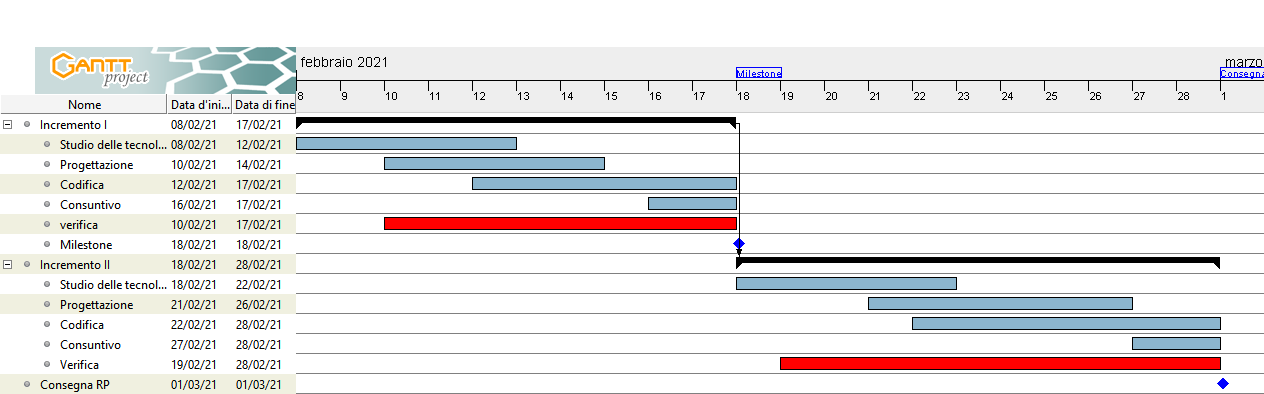
\includegraphics[width=\linewidth]{Images/GanttPianificazioneProgettazionePoc.PNG}
	\caption{Diagramma di Gantt dell'attività di progettazione e codifica del Proof Of Concept}
\end{figure}





\newpage
\subsection{Progettazione di dettaglio e codifica}
Questa fase comincia in seguito a quella precedente e termina con la \textit{Revisione di Qualifica}, ovvero dal 08-03-2021 al 02-04-2021. Durante questa fase verranno implementate buona parte delle componenti della web app e verranno anche aggiunte funzionalità alle componenti già sviluppate in precedenza.
Di seguito è riportato il dettaglio di ogni incremento.

\subsubsection{Incremento III}
\textit{dal 08-03-2021 al 13-03-2021}\\
L'incremento III prevede la progettazione di dettaglio e codifica delle componenti software. Si prevede di svolgere quanto segue:
\begin{itemize}
\item Implementazione di un componente per applicare una riduzione dimensionale ai dati;
\item Aggiunta di alcuni controlli per la configurazione dei parametri relativi ai diversi algoritmi di riduzione dimensionale disponibili.
\end{itemize}
\textbf{Attività}
\begin{itemize}
\item \textbf{Stesura:} eventuali correzioni ai documenti ed inizio stesura dell'allegato tecnico con scelta dei design patterns;
\item \textbf{Verifica documenti}
\item \textbf{Progettazione:} progettazione del componente per la riduzione dimensionale;
\item \textbf{Codifica:} codifica del componente per la riduzione dimensionale con relativa parametrizzazione;
\item \textbf{Verifica software:} verifica sulle funzionalità software aggiunte.
\end{itemize}
\subsubsection{Incremento IV}
\textit{dal 13-03-2021 al 17-03-2021}\\
L'incremento IV prevede la progettazione di dettaglio e codifica delle componenti software. Si prevede di svolgere quanto segue:
\begin{itemize}
\item Implementazione della visualizzazione Heat Map;
\item Aggiunta di alcuni controlli per la configurazione dei parametri relativi alla visualizzazione precedentemente implementata.
\end{itemize}
\textbf{Attività}
\begin{itemize}
\item \textbf{Stesura:} incremento della documentazione da allegare al prodotto;
\item \textbf{Verifica documenti}
\item \textbf{Progettazione:} progettazione del componente per la visualizzazione Heat Map;
\item \textbf{Codifica:} codifica del componente per la visualizzazione con relativa parametrizzazione;
\item \textbf{Verifica software:} verifica sulle funzionalità software aggiunte.
\end{itemize}

\subsubsection{Incremento V}
\textit{dal 17-03-2021 al 21-03-2021}\\
L'incremento V prevede la progettazione di dettaglio e codifica delle componenti software. Si prevede di svolgere quanto segue:
\begin{itemize}
\item Implementazione della visualizzazione Force Field;
\item Aggiunta di alcuni controlli per la configurazione dei parametri relativi alla visualizzazione precedentemente implementata.
\end{itemize}
\textbf{Attività}
\begin{itemize}
\item \textbf{Stesura:} incremento della documentazione da allegare al prodotto e inizio del manuale utente e del manuale manutentore;
\item \textbf{Verifica documenti}
\item \textbf{Progettazione:} progettazione del componente per la visualizzazione Force Field;
\item \textbf{Codifica:} codifica del componente per la visualizzazione con relativa parametrizzazione;
\item \textbf{Verifica software:} verifica sulle funzionalità software aggiunte.
\end{itemize}

\subsubsection{Incremento VI}
\textit{dal 21-03-2021 al 26-03-2021}\\
L'incremento V prevede la progettazione di dettaglio e codifica delle componenti software. Si prevede di svolgere quanto segue:
\begin{itemize}
\item Implementazione della visualizzazione Proiezione Lineare Multi Asse;
\item Aggiunta di alcuni controlli per la configurazione dei parametri relativi alla visualizzazione precedentemente implementata.
\end{itemize}
\textbf{Attività}
\begin{itemize}
\item \textbf{Stesura:} incremento della documentazione da allegare al prodotto ;
\item \textbf{Verifica documenti}
\item \textbf{Progettazione:} progettazione del componente per la visualizzazione Proiezione Lineare Multi Asse;
\item \textbf{Codifica:} codifica del componente per la visualizzazione con relativa parametrizzazione;
\item \textbf{Verifica software:} verifica sulle funzionalità software aggiunte.
\end{itemize}

\subsubsection{Incremento VII}
\textit{dal 26-03-2021 al 2-04-2021}\\
L'incremento V prevede la progettazione di dettaglio e codifica delle componenti software. Si prevede di svolgere quanto segue:
\begin{itemize}
\item Implementazione di un database;
\item Sviluppo di un componente per la scelta e il caricamento di un dataset contenuto nel database.
\end{itemize}
\textbf{Attività}
\begin{itemize}
\item \textbf{Stesura:} incremento e conclusione della documentazione da allegare al prodotto ;
\item \textbf{Verifica documenti}
\item \textbf{Progettazione:} progettazione del database e del componente per la scelta e il caricamento del dataset;
\item \textbf{Creazione struttura database:} stesura della struttura del database;
\item \textbf{Codifica:} codifica del componente per la scelta e il caricamento del dataset;
\item \textbf{Verifica software:} verifica sulle funzionalità software aggiunte.
\end{itemize}

\begin{landscape}

\begin{figure}[h]
 	\centering
	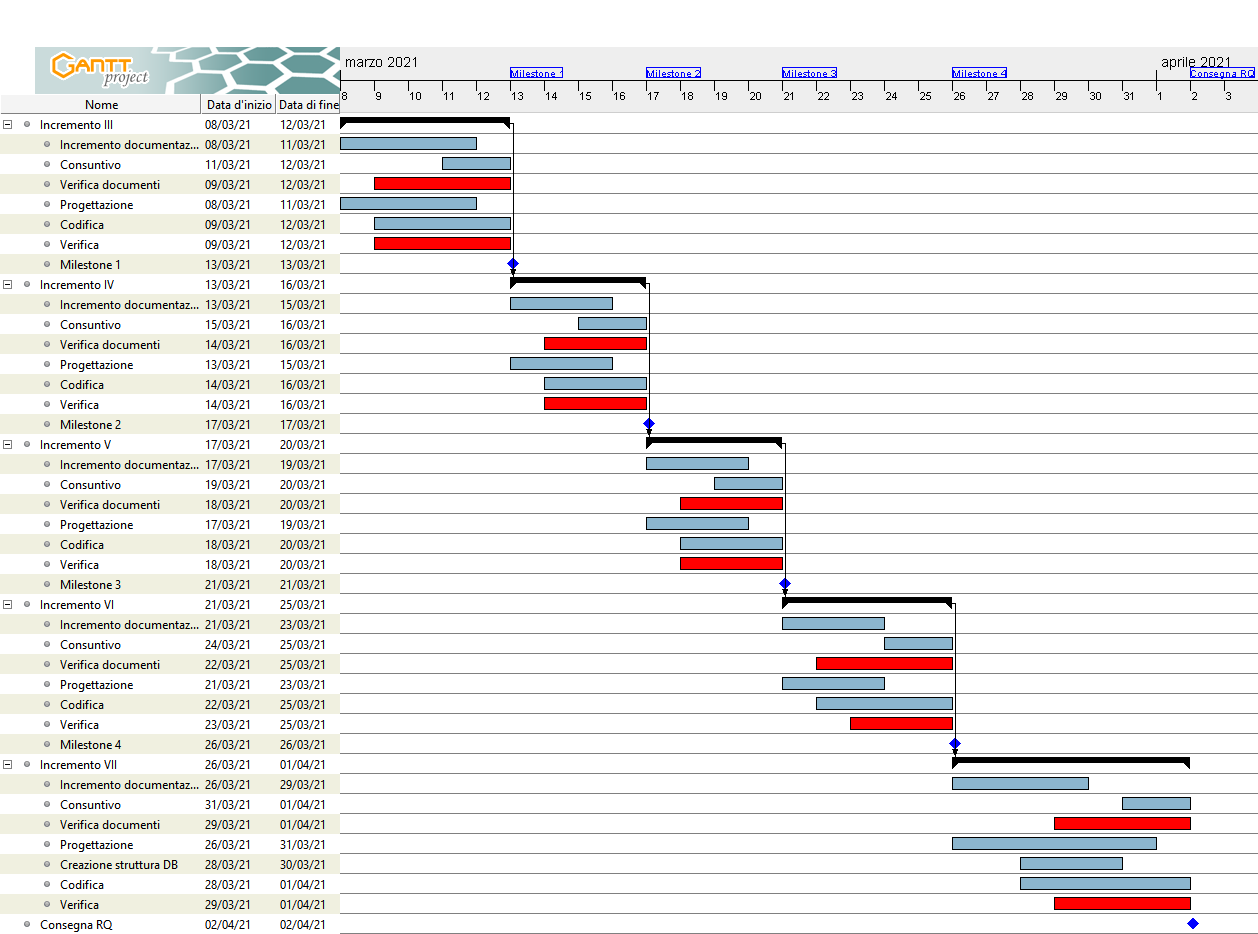
\includegraphics[width=\linewidth]{Images/GanttPianificazioneProgettazioneDettaglioCodifica.png}
	\caption{Diagramma di Gantt dell'attività di Progettazione di dettaglio e Codifica}
\end{figure}

\end{landscape}
\newpage
\subsection{Completamento e raffinamento delle funzionalità}
Questa fase comincia subito dopo la consegna dei documenti per la \textit{Revisione di Qualifica}, ovvero il 26-04-2021 e termina il 30-04-2021.\\
In questo periodo verranno creati ulteriori test per verificare il corretto funzionamento del prodotto. Se tutte le scadenze imposte dal gruppo vengono rispettate il tempo in eccesso viene occupato per la realizzazione di requisiti opzionali, concordati con il proponente. 

\subsubsection{Incremento VIII} 

\paragraph{Obiettivi}
\begin{itemize}
	\item Implementazione della gestione della sessione;
	\item Implementazione di un componente per l'esportazione dei parametri di configurazione dell'applicazione \textbf{[UC7]};
	\item Implementazione di un componente per l'importazione dei parametri di configurazione dell'applicazione \textbf{[UC1.2]}.
\end{itemize}
	
\paragraph{Periodi e attività} \mbox{}\\\mbox{}\\
Questo incremento si compone di un unico periodo, dal  26-04-2021 al 30-04-2021, con milestone fissata per l'ultimo giorno. Comprende attività di:	
\begin{itemize}
\item \textbf{Stesura:} incremento della documentazione da allegare al prodotto;
\item \textbf{Verifica dei documenti};
\item \textbf{Progettazione:} progettazione di un sistema per la gestione della sessione;
\item \textbf{Codifica:} codifica dei componenti per l'importazione e l'esportazione dei parametri di configurazione dell'applicazione;
\item \textbf{Verifica software:} verifica sulle funzionalità software aggiunte.
\end{itemize}
%
%\subsubsection{Incremento IX} 
%
%\paragraph{Obiettivi}
%\begin{itemize}
%	\item Implementazione di un sistema di \glo{widget} per l'utilizzo dell'applicazione;
%	\item Realizzazione una guida introduttiva per l'utilizzo dell'applicazione.
%\end{itemize}			
%\paragraph{Periodi e attività} \mbox{}\\\mbox{}\\
%Questo incremento si compone di un unico periodo, dal  16-04-2021 al 23-04-2021, con milestone fissata per l'ultimo giorno.		
%\begin{itemize}
%\item \textbf{Stesura:} incremento della documentazione da allegare al prodotto;
%\item \textbf{Verifica dei documenti} 
%\item \textbf{Progettazione:} progettazione di un sistema di \glo{widget} e di una guida introduttiva;
%\item \textbf{Codifica:} codifica dei componenti per i \glo{widget} e per la guida introduttiva;
%\item \textbf{Verifica software:} verifica sulle funzionalità software aggiunte.
%\end{itemize}

\begin{figure}[h]
	\centering
	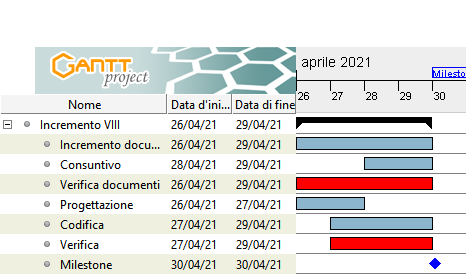
\includegraphics[width=12cm]{Images/GanttPianificazioneRaffinamentoFunzionalita.PNG}
	\caption{Diagramma di Gantt dell'attività di completamento e raffinamento delle funzionalità}
\end{figure}
\newpage
\subsection{Validazione e Collaudo}
Questa fase comincia subito dopo la fase precedente e finisce con la data di consegna per la \textit{Revisione di Accettazione}, ovvero dal 09-04-2020 al 03-05-2020.\\
In questo periodo verranno creati ulteriori test per verificare il corretto funzionamento del prodotto. Se tutte le scadenze imposte dal gruppo vengono rispettate il tempo in eccesso viene occupato per la realizzazione di requisiti opzionali, concordati con il committente. 
\subsubsection{Attività}
\begin{itemize}
\item \textbf{Incremento e verifica dei documenti:} se fosse necessario, i documenti prodotti dal team verranno integrati.

 \item \textbf{Incremento e verifica delle attività}: sia la \textit{Technology baseline} che la \textit{Product Baseline} vengono eventualmente raffinate; particolare attenzione va alla codifica, svolta ad incrementi ciclici.
 \begin{itemize}
 \item \textbf{Incremento X}: il gruppo identifica e implementa la soluzione più adeguata per la gestione della sessione nell'applicazione. Incremento della documentazione da correlare al prodotto software e incremento della documentazione per verifica e miglioramento continuo \textbf{[UC1.2, UC7]};
\item \textbf{Incremento XI}: viene perfezionato il codice precedentemente, il prodotto viene collaudato e vengono vericati tutti i documenti precedentemente redatti. 
 \end{itemize}

 \item \textbf{Verifica e collaudo}: vengono creati e applicati un set di test, che hanno lo scopo di portare il prodotto ad un buon livello qualitativo. Il gruppo si focalizzerà sulla sua correttezza e nel rispetto di tutti i requisiti.
\end{itemize}

\subsubsection{Periodi}
La pianificazione di questa fase è stata organizzata con le seguenti milestone:

\begin{itemize}
\item \textbf{Periodo 1}: \textit{(dal 09-04-2020 al 16-04-2020)} se fosse necessario, in questo periodo viene controllata tutta la documentazione e ci si dedicherà ad eventuali incrementi della \textit{Technology Baseline} e \textit{Product Baseline}, è fissata una milestone l'ultimo giorno di questo periodo entra cui dovrà essere terminato l'incremento X.

\item \textbf{Periodo 2}: \textit{(dal 16-04-2020 al 03-05-2020)} entro la milestone del 03-05-2020 il gruppo ha come obbiettivo quello di completare l'ultimo incremento.

\end{itemize}
\newpage
\subsubsection{Diagramma di Gantt: Validazione e Collaudo}
\begin{figure}[h]
	\centering
	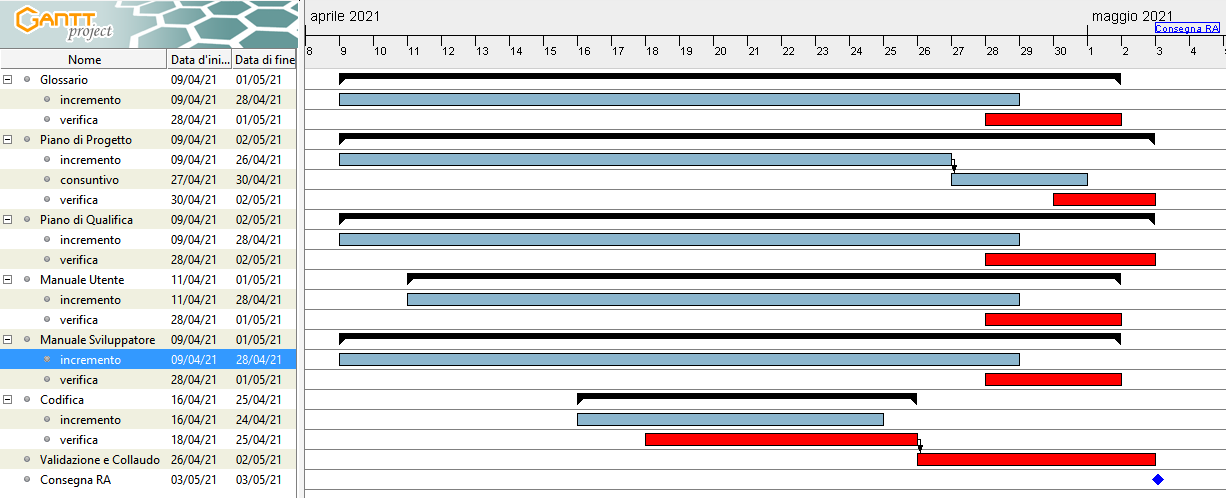
\includegraphics[scale=0.5]{Images/GanttValidazioneCollaudo.PNG}
	\caption{Diagramma di Gantt dell'attività di Validazione e Collaudo}
\end{figure}